\section{Implementierung von Polynomen}
\label{sec:polynomials}
\texttt{GalFld/Core/Polynomials.hs}\\
\texttt{GalFld/Core/Polynomials/FFTTuple.hs}\\
\texttt{GalFld/Core/Polynomials/Conway.hs}\\

\subsection{Der Datentyp}

Grundsätzlich gibt es zwei verschiedene Möglichkeiten Polynome zu
implementieren: \emph{sparse} und \emph{dense}, d.h. 
\begin{itemize}
  \item entweder entscheidet man
    sich, ein Polynom $f(X) = a_nX^n + \ldots + a_0$ als Liste\footnote{Was genau 
    eine ,,Liste`` in der jeweilig benutzten Sprache bedeuten soll, bleibt der
    Interpretation überlassen.} der Länge $n+1$ zu hinterlegen,
  \item oder man speichert lediglich eine Liste von Tupeln $(i,a_i)$, sodass
    $i \in \{0,\ldots,n\}$ den Index/Exponenten des Koeffizienten $a_i$ angibt
    und alle Koeffizienten, die Null sind, ausgelassen werden.
\end{itemize}
In der hier vorliegenden finalen Implementierung haben wir uns für letztere
Variante entschieden, da diese insbesondere bei spärlich besetzten Polynomen
mit hohem Grad deutliche Performancegewinne zeigt.

Konkret ist ein Polynom also definiert durch:
\haskellinput{Core/Polynomials}{data Polynom}

Um diese Darstellung \emph{dense} nennen und mit ihr effizient arbeiten zu 
können, legen wir folgende Beschränkungen für die Implementierung fest:
\begin{invariante}
  \label{inv:poly}
  Für ħPMS $L$ Trueħ gilt stets, dass die Monome in $L$ alle nicht Null 
  sind und ihrem Grade nach in
  absteigender Reihenfolge sortiert sind, d.h.
  \begin{enumerate}
    \item für alle $(i,x) \in L$ ist $x \neq 0$.
    \item für alle $(i,x), (j,y) \in L$ gilt: Steht $(i,x)$ vor $(j,y)$, so ist
      $i > j$.
  \end{enumerate}
  Ein Polynom, das diese Eigenschaften erfüllt, wollen wir auch 
  \emph{wohlgeformt} oder \emph{korrekt dargestellt} nennen.
\end{invariante}

\begin{beispiel}
  Für das Polynom $f(X) = X^5 + 3X^2 + 1$ wäre 
  \begin{hcode}
    PMS [(5,1), (2,3), (0,1)] True
  \end{hcode}
  die korrekte Darstellung.
\end{beispiel}

Damit diese Invariante stets sichergestellt ist, existiert die Funktion
ħcleanPħ, mit der eine ħ[(Int,a)]ħ Liste in die korrekte Form gebracht werden
kann:
\haskellinput{Core/Polynomials}{cleanP}

\subsection{Instanzen}
Es wurden die offensichtlichen Instanzen implementiert, d.h.
ħEqħ und ħNumħ. Zudem wurden zur Anzeige von Polynomen ħShowħ und ħShowTexħ, zur
binären Speicherung ħBinaryħ und für eine Auswertung trotz Lazyness ħNFDataħ
implementiert.

Alle auftauchenden Funktionen werden im weiteren Verlauf näher erläutert.

\paragraph{Eq}\makebox{} 
\haskellinput{Core/Polynomials}{instance .*?=> Eq}

\paragraph{Num}\makebox{}  
\haskellinput{Core/Polynomials}{instance .*?=> Num}
    
\paragraph{Show}\makebox{}  
\haskellinput{Core/Polynomials}{instance .*?=> Show}

\paragraph{ShowTex}\makebox{}  
\haskellinput{Core/Polynomials}{instance .*?=> ShowTex}

\subsection{Polynome erstellen}
\paragraph{Allgemein}
\thref{inv:poly} erfordert auch, dass der Konstruktor des Polynomdatentyps
nicht öffentlich gemacht wird und wir benötigen separate Funktionen, um
Polynome zu erstellen. Diese sind selbsterklärend:
\haskellinput{Core/Polynomials}{pList}
\haskellinput{Core/Polynomials}{pTup}
Ferner existiert noch eine Variante der ,,unsicheren`` Erstellung von
Polynomen, die eine korrekte Darstellung nach \thref{inv:poly} voraussetzt,
diese jedoch nicht prüft. 
\haskellinput{Core/Polynomials}{pTupUnsave}


\paragraph{Polynome dekonstruieren}
Den Weg rückwärts zu gehen ist natürlich auch möglich, was ħp2Tupħ und ħp2Listħ
bewerkstelligen:

\haskellinput{Core/Polynomials}{p2Tup}
\haskellinput{Core/Polynomials}{p2List}


\paragraph{Spezielle Polynome}
Eines der am häufigsten verwendeten Polynome ist das Nullpolynom. Daher gibt
es sowohl eine Prüfung, ob ein Polynom null ist, als auch das Nullpolynom
selbst als Objekt:
\haskellinput{Core/Polynomials}{nullP}
\haskellinput{Core/Polynomials}{isNullP}


Des Weiteren haben wir eine kleine Schreibhilfe zur Erstellung von konstanten
Polynomen generiert:
\haskellinput{Core/Polynomials}{pKonst}

\subsection{Einwertige Operationen auf Polynomen}

\paragraph{Der Grad} Der Grad eines Polynoms, lässt sich aufgrund 
\thref{inv:poly} sehr leicht herausfinden. Es gilt jedoch zu beachten, dass der
Grad des Nullpolynoms nicht $0$ ist. Wir haben uns daher entschieden, den Grad
als ħMaybe Intħ zu implementieren:
\haskellinput{Core/Polynomials}{degP}
Es ist klar, dass man meistens einen ħIntħ als Grad haben möchte, daher haben
wir folgende Funktion implementiert:
\haskellinput{Core/Polynomials}{uDegP}

\paragraph{Auswerten} Natürlich muss man auch etwas in ein Polynom einsetzen
können, was wir mit Hilfe des Horner-Schemas (vgl.
\autocite{wiki:horner-schema})
implementiert haben. Dies zeigt eine schöne Anwendung der Haskellfunktion 
ħfoldlħ:
\haskellinput{Core/Polynomials}{evalP}


\paragraph{Normieren} Über das Normieren braucht man nicht viele Worte
verlieren.
\haskellinput{Core/Polynomials}{moniP}
Da man in vielen Situationen das Inverse des Leitkoeffizienten des Polynoms 
bei der Normierung erhalten möchte, gibt es noch die folgende Variante der Normierung:
\haskellinput{Core/Polynomials}{moniLcP}

\paragraph{Formale Ableitung} \makebox{ }
\haskellinput{Core/Polynomials}{deriveP}

\paragraph{Das reziproke Polynom} 
\begin{definition}[reziprokes Polynom]
  \label{def:reziprokesPoly}
  Sei $f(X) = \sum_{i=0}^n a_i X^i \in R[X]$ für einen Körper $R$, so ist 
  das \emph{reziproke Polynom von Ordnung $d$ von $f(X)$} für $d \geq n$ 
  gegeben durch
  \[ f^\ast_d(X) := X^d f(\tfrac{1}{X})\,.\]
\end{definition}

\haskellinput{Core/Polynomials}{reciprocP2}

Das reziproke Polynom, wie man es normalerweise kennt, ist dann für $d=n$ in
obiger Definition gegeben durch

\haskellinput{Core/Polynomials}{reciprocP}


\paragraph{Multiplikation mit Monomen}
Es ist klar, dass die Multiplikation eines Polynoms mit einem Monom einfacher
ist, als der allgemeine Fall. Daher verdient dieses Vorgehen eine eigene
Funktion:

\haskellinput{Core/Polynomials}{multMonomP}




\subsection{Zweiwertige Operationen auf Polynomen}
\paragraph{Gleichheit} Bekanntlich sind zwei Polynome 
genau dann gleich, wenn ihre Koeffizienten übereinstimmen:
\haskellinput{Core/Polynomials}{eqP}


\paragraph{Addition} Hier kommt zum ersten Mal ein kleiner Nachteil der
\emph{dense} Darstellung zu Tage, da das Addieren zweier Polynome nicht einfach
das elementweise Summieren zweier Listen ist, sondern stets geprüft werden
muss, bei welchem Grad man gerade ist:
\haskellinput{Core/Polynomials}{addPM}
ħaddPMħ darf offensichtlich nur ausgeführt werden, wenn die beiden Polynome
\thref{inv:poly} erfüllen. Darüber hinaus stellt obige Funktion auch sicher,
dass besagte Invariante erhalten bleibt.

\paragraph{Subtraktion} Da die funktionale Programmierung lediglich 
nicht veränderbare Objekte (\emph{immutable objects}) vorsieht, würde durch die
Standarddefinition der Subtraktion, nämlich Addition des ersten mit dem
negierten zweiten Argument, das zweite Polynom doppelt durchlaufen (einmal beim
Negieren und einmal beim Addieren). Um dies zu verhindern, haben wir die
Subtraktion separat geschrieben.
\haskellinput{Core/Polynomials}{subtrPM}
Wiederum darf obige Subtraktion nur auf wohlgeformte Polynome angewandt werden.

\paragraph{Multiplikation}
Es hat sich herausgestellt, dass in den meisten Fällen die 
,,Standardmultiplikation`` die effizienteste ist. Diese ist wie folgt
implementiert:
\haskellinput{Core/Polynomials}{multPM}
\haskellinput{Core/Polynomials}{multPM'\string\''}
Wir haben jedoch auch die Multiplikation nach Karatsuba und eine Multiplikation
auf FFT-Grundlage implementiert, wie in \autoref{subsec:multAlgs} nachzulesen ist.

\paragraph{Division mit Rest}
Wie auch schon bei der Multiplikation von Polynomen, kennt man bei der Division
mit Rest verschiedene Algorithmen. Als erste und einfachste Wahl bietet sich
die Division mit Rest nach Grundschulmethode an. Diese hat sich jedoch als
langsamste erwiesen und wurde daher wieder aus dem Code entfernt. Die nun in
den meisten Fällen schnellste Methode ist die Division mit Hilfe des
Horner-Schemas. Eine sehr gute und ausführliche Erklärung findet sich 
in \autocite{wiki:synthetic-division}.

Wiederum lässt sich die Division per Horner-Schema sehr schön rekursiv in
Haskell niederschreiben.
\haskellinput{Core/Polynomials}{divPHornerM'\string\''}

Wie in den obigen Funktionen kommt man auch hier nicht ohne Overhead aus, der
notwendig ist, um die verschiedenen Polynom-Status (ħcleanPħ betreffend) zu
behandeln und die initialen Parameter festzulegen.
\haskellinput{Core/Polynomials}{divP}
\haskellinput{Core/Polynomials}{divPHorner}

\paragraph{,,Division``} Für den Fall, dass man bereits weiß, dass ein
Polynom durch ein anderes teilbar ist, haben wir den Operator ħ(@/)ħ definiert
\footnote{Zu beachten ist hierbei, dass die Benutzung 
von \lstinline{(/)}nicht möglich 
ist, da es eine \lstinline{Fractional}-Instanz erfordern würde, 
die es auf Polynomen ja offenbar nicht gibt.}.
Dieser ist selbstredend nichts anderes als Division mit Rest, wobei lediglich
der erste Eintrag des Tupels zurückgegeben wird.

% TODO
%\haskellinput{Core/Polynomials}{(\string\@\string\/)}


\paragraph{Modulo} Dual zu ħ(@/)ħ ist ħmodByPħ, das einfach den zweiten Eintrag
von ħdivPħ liefert:

\haskellinput{Core/Polynomials}{modByP}


\paragraph{Erweiterter Euklidischer Algorithmus} Auch der erweiterte
Euklidische Algorithmus basiert auf ħdivPħ. Er ist -- selbstverständlich
rekursiv -- hier gegeben durch:

\haskellinput{Core/Polynomials}{eekP}

\paragraph{Größter gemeinsamer Teiler} Aus dem erweiterten Euklidischen
Algorithmus erhält man selbstverständlich auch den $\ggT$ zweier Polynome:

\haskellinput{Core/Polynomials}{ggTP}

\subsection{Weiteres}

\paragraph{Nullstellensuche} Möchte man prüfen, ob ein Polynom in einer
gewissen Menge von Elementen eine Nullstelle besitzt, so ist dies mit folgender
Funktion möglich.

\haskellinput{Core/Polynomials}{hasNs}

\paragraph{Auflisten aller Polynome} 
Folgende Funktion listet alle monischen Polynome auf, deren Grad in der Liste
ħ[Int]ħ vorkommt und deren Koeffizienten in der Liste ħ[a]ħ liegen.

\haskellinput{Core/Polynomials}{getAllMonicPs}

Möchte man Polynome von Grad $0$ bis zu einem gewissen Grad, so liefert dies
die Funktion ħgetAllMonicPħ.

\haskellinput{Core/Polynomials}{getAllMonicP}

Zuletzt kann man sich natürlich noch zusätzlich die nicht-monischen Polynome
ausgeben lassen; wie oben in beiden Varianten (d.h. Grade als Liste oder als
Obergrenze gegeben).

\haskellinput{Core/Polynomials}{getAllPs}
\haskellinput{Core/Polynomials}{getAllP}

\paragraph{Conway-Polynome}
Die \emph{Conway-Polynome} bieten in gewisser Weise eine kanonische Möglichkeit
Körpererweiterungen endlicher Körper zu charakterisieren. Für Definitionen
und Eigenschaften sei auf
\url{http://www.math.rwth-aachen.de/~Frank.Luebeck/data/ConwayPol/index.html}
verwiesen, wo auch die Conway-Polynome zu finden sind, die wir in der Datei
\texttt{GalFld/Core/Polynomials/Conway.hs} hinterlegt haben.




\section{Alternative Polynomalgorithmen}
\subsection{Verschiedene Multiplikationsalgorithmen}
\label{subsec:multAlgs}

\subsubsection{Karatsuba}
Einer der häufigsten Multiplikationsalgorithmen für Polynome ist sicher der
Karatsuba. Er basiert auf der Idee, Multiplikationen durch Additionen zu
ersetzen, die im Allgemeinen ,,billiger`` sind. 

Der Basisfall für die Multiplikation zweier Polynome von Grad 1 lässt die Idee
des Algorithmus deutlich werden:
\[ (a_1 X + b_1) \cdot (a_2 X + b_2) = 
  A X^2 + (C - A - B) X + B\]
wobei 
\[ A = a_1 b_1, \qquad B = a_2b_2, \qquad C = (a_1+b_1)(a_2+b_2) \,.\]
Damit können die ursprünglich 4 auftretenden Multiplikationen des
Standardalgorithmus durch 3 Multiplikationen und 4 Additionen ersetzt werden.
Dies lässt sich natürlich rekursiv anwenden. Da die Polynome jedoch nicht immer
gleichen Grades sind und dieser selten eine Zweierpotenz ist (letzteres ist
notwendig, damit der Algorithmus rekursiv bis zu obigem Grundfall laufen kann),
wählt man die nächstkleinere Zweierpotenz des Maximums der beiden Grade als
Teilungspunkt für den rekursiven Aufruf.
Die Implementierung erfolgt dabei in drei Schritten: 
\haskellinput{Core/Polynomials}{multPK}
Hierzu gibt es nichts zu sagen. Im nächsten Schritt wird dann die passende
Zweierpotenz ermittelt und damit der eigentliche Karatsuba aufgerufen:
\haskellinput{Core/Polynomials}{multPMKaratsuba}
Letztlich bleibt nur der Algorithmus übrig. Aufgrund der Tupeldarstellung der
Polynome, ist die Trennung selbiger nicht so einfach und elegant, wie es die
Listendarstellung erlaubt hätte. Nichtsdestotrotz ist diese Implementierung
auch in diesem Fall effizienter.
\haskellinput{Core/Polynomials}{multPMK'\string\''}

\paragraph{Ein kleiner Vergleich}
Auf Polynomen über den ħPrimeFieldsħ bringt der Karatsuba erst bei sehr hohen
Graden einen leichten Vorteil gegenüber der Standardmultiplikation. 
Betrachten wir jedoch
ein Beispiel über einem Erweiterungskörper, so kann der Karatsuba seinen Vorteil
ausspielen, da dort ja die Koeffizienten selbst Polynome sind, und daher
Addition weitaus ,,billiger`` ist als Multiplikation.
\autoref{fig:karavsnorm} zeigt dies deutlich.

\begin{figure}
  \caption{Vergleich von normaler Multiplikation mit Karatsuba}
  \label{fig:karavsnorm}
  \centering
  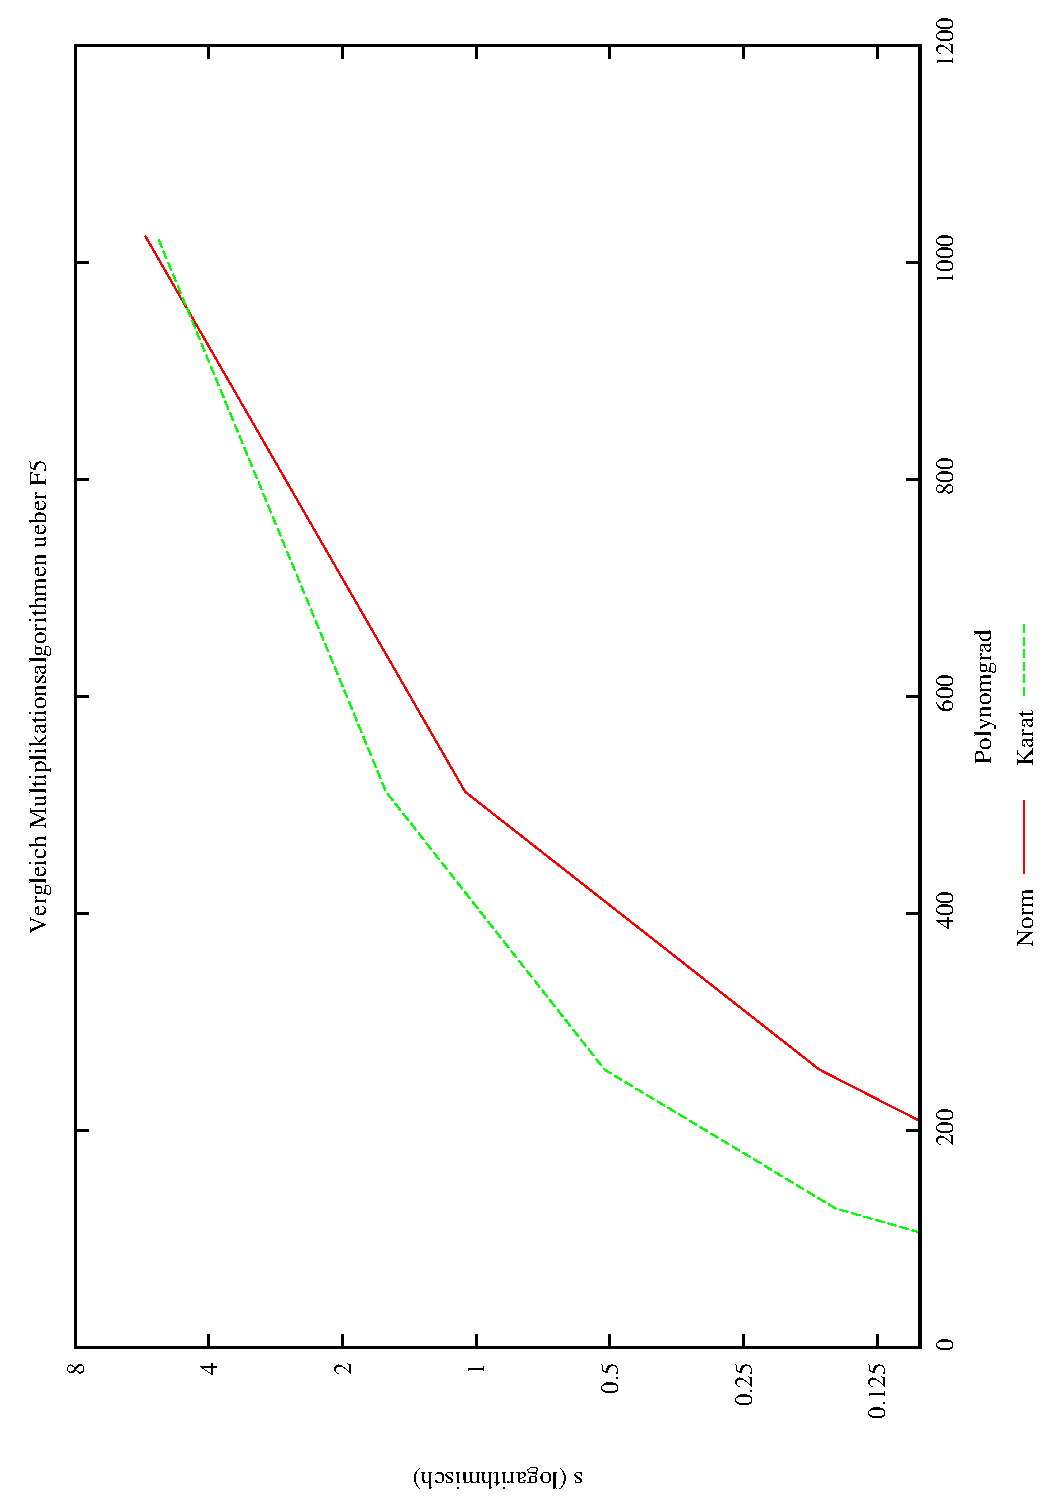
\includegraphics[angle=-90,width=0.7\textwidth]{plots/benchNormVsKara_F5.pdf}
  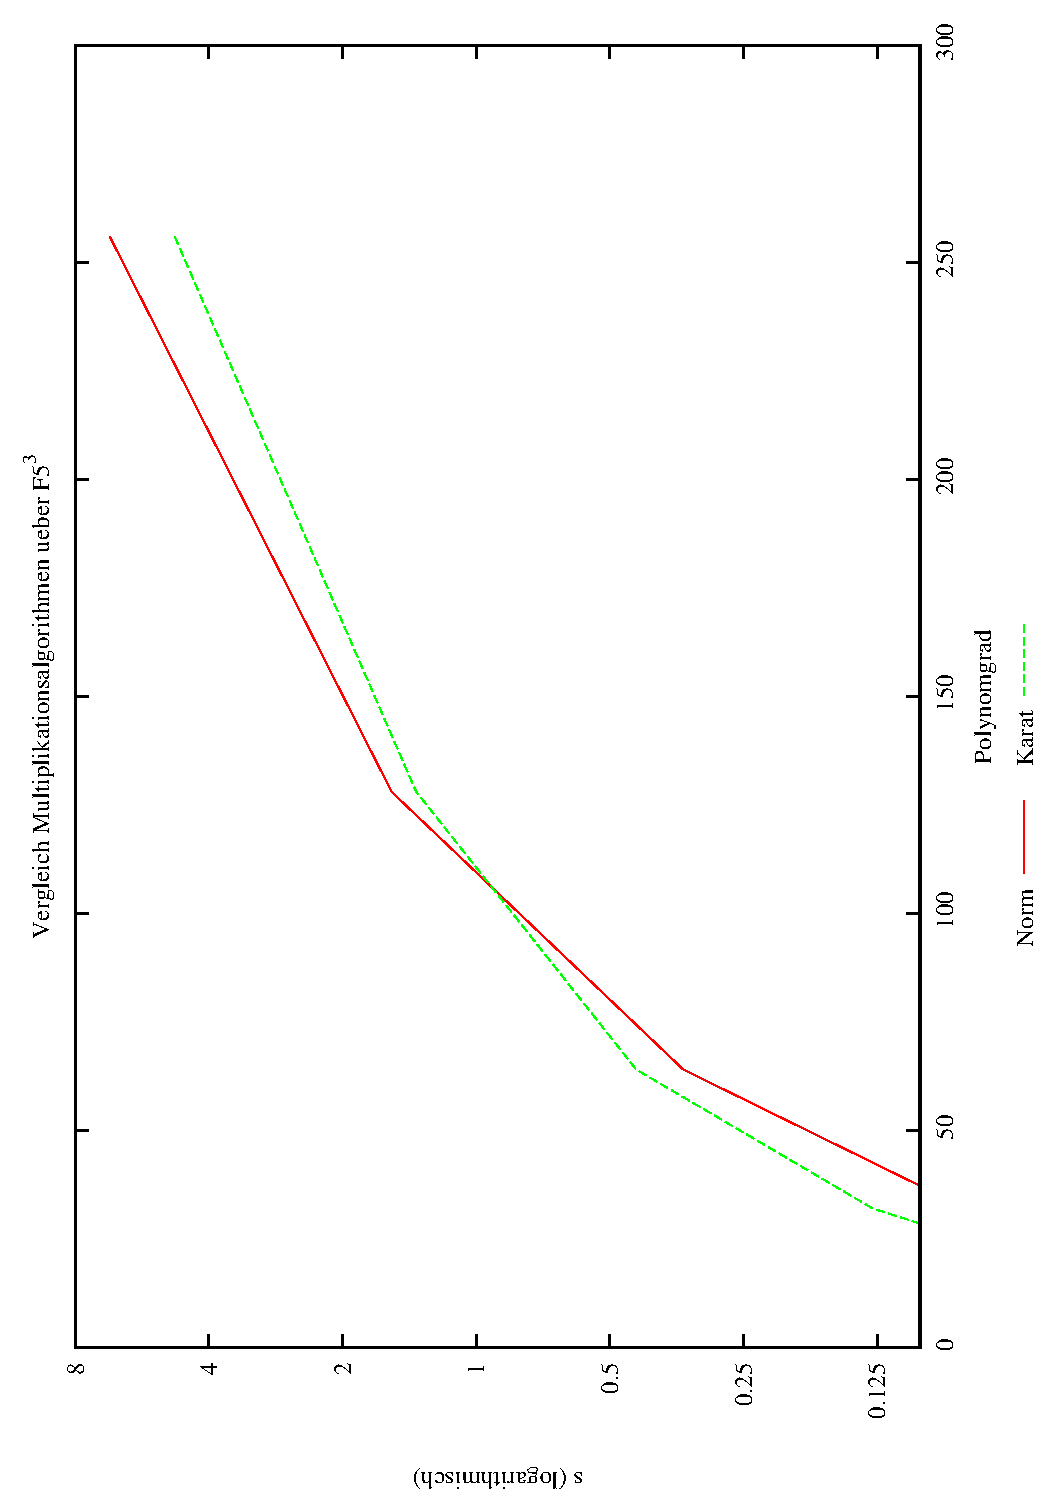
\includegraphics[angle=-90,width=0.7\textwidth]{plots/benchNormVsKara_F53.pdf}
\end{figure}


\subsubsection{FFT-Multiplikation: Der Schönhage-Strassen-Algorithmus}
Eine der Idee nach weitaus komplexere Möglichkeit Polynome zu
multiplizieren, ist die Multiplikation auf Basis der schnellen
Fourier-Transformation (engl. \emph{fast Fourier transform} (FFT)). 
Sie ist die bislang schnellste
bekannte Methode. Allerdings gilt dies nur für die asymptotische Laufzeit!
Daher konnten wir leider nur feststellen, dass die FFT-Multiplikation stets
weitaus langsamer ist, als der Standardalgorithmus oder Karatsuba.

Die Idee der FFT-Multiplikation basiert auf der Tatsache, dass sich das Produkt
zweier Polynome in diskreter Fourier-Transformation (DFT) als komponentenweises
Produkt der Fourier-Transformierten beider Polynome berechnen lässt. 
Dies wollen wir uns näher betrachten:

Im Folgenden sei stets $R$ ein kommutativer Ring mit Eins und 
$\omega\in R$ eine primitive $n$-te Einheitswurzel.

\begin{definition}
   Ist $f\in R[X]$ ein Polynom, so ist seine
  \emph{diskrete Fourier-Transformation (DFT)} definiert als
  \[ f^\wedge(\omega) = (f(\omega^j):\ j=0,\ldots,n-1) \in R^n\,.\]
\end{definition}

Eine wesentliche Eigenschaft liefert folgende Proposition. 

\begin{prop}
  Sei $f \in R[X]$ und $F := f^\wedge(\omega)$ seine DFT. Ist 
  $n \in R$ eine Einheit, so gilt
  \[ f(X) = (\tfrac 1 n F^\wedge(\omega^{-1}))(X) \,.\]
\end{prop}
\begin{proof}
  \autocite[Proposition 4.9]{fft}. 
\end{proof}

Die auftauchende Frage zur Notation eines $n$-Tupels als Polynom beantwortet
nachstehende Definition:

\begin{definition}
  Sei $r = (r_0,\ldots,r_{n-1})\in R^n$, so definieren wir 
  \[ r(X) := \sum_{i=0}^{n-1} r_i X^i \ \in R[X] \,.\]
  Ferner notieren wir für 
  $f(X) = \sum_{i=0}^{n-1} f_i X^i \in R[X]$
  \[ f = (f_0,\ldots,f_{n-1}) \in R^n \,.\]
\end{definition}

Die DFT eines Polynoms lässt sich sehr schnell durchführen, wenn man
$n = 2^l$ eine Zweierpotenz setzt:
\begin{pseudocode}{FFT}{alg:fft}
Input: $n = 2^l$, $\omega \in R$ eine primitive $n$-te Einheitswurzel, $f \in R^n$
Output: $f^\wedge(\omega)$
Algorithmus FFT($n$,$\omega$,$f$):
  1. Setze
    $r := \big(f_j + f_{j+\frac n 2}:\ j=0,\ldots,\tfrac n 2\big)$
    $r_\omega := \big( \omega^j (f_j - f_{j+\frac n 2}):\
         j=0,\ldots,\tfrac n 2\big)$
  2. Berechne rekursiv $a := $ FFT($\tfrac n 2$, $\omega^2$, $r$) und $b := $ FFT($\tfrac n 2$, $\omega^2$, $r_\omega$)
  3. Mische die Ergebnisse: $f^\wedge(\omega) := (a_0,b_0,a_1,\ldots,
      a_{\frac n 2 -1},b_{\frac n 2 -1})$
\end{pseudocode}

Wie man damit Polynome multiplizieren kann, erklärt nachstehender Algorithmus:
\begin{pseudocode}{FFT-Multiplikation}{alg:dftmul}
Input: $\omega \in R$ eine primitive $n$-te Einheitswurzel, $n = 2^l$,
       $f(X),g(X) \in R[X]$ mit $\deg f + \deg g < n$
Output: $h(X) = f(X)g(X) \in R[X]$
Algorithmus FFTM($f$,$g$,$n$,$\omega$):
  1. Berechne $a := f^\wedge(\omega)$, $b := g^\wedge(\omega)$.
  2. Berechne komponentenweise $c := a\odot b$.
  3. Setze $h(X) := (\tfrac 1 n c^\wedge(\omega\inv))(X)$
\end{pseudocode}


Es bleiben ein paar Probleme offen: Um mit obigem Algorithmus Polynome zu
multiplizieren, muss in $R$ für jede Zweierpotenz $n$ eine primitive $n$-te
Einheitswurzel existieren und $2$ eine Einheit sein. Die Tatsache, dass 2 eine
Einheit sein muss, spielt für den Fall der Anwendung -- nämlich Multiplikation 
von Polynomen über endlichen Körpern -- quasi keine Rolle, da für
Charakteristik ungleich 2 dies dort ja immer 
gegeben ist.\footnote{Für Charakteristik 2 existieren ohnehin spezielle
Algorithmen auf Basis von Binäroperationen!}
Jedoch bleibt offen, wie man eine $n$-te Einheitswurzel finden 
soll.  Die allgemeine Antwort lautet in diesem Fall: Wir suchen gar nicht, 
sondern modifizieren das Setting so, dass stets eine $n$-te Einheitswurzel 
gegeben ist:

\begin{lemma}
  Sei $R$ ein kommutativer Ring und $2 \in R$ eine Einheit. Sei ferner
  $n = 2^l$ mit $l\geq 1$. Dann ist 
  \[ \omega := X\  \in\ R_n := R[X]\big/(X^n+1)\]
  eine primitive $(2n)$-te Einheitswurzel.
\end{lemma}
\begin{proof}
  \autocite[Lemma 4.15]{fft}.
\end{proof}

Das bedeutet, wir ,,erzwingen`` die Existenz einer passenden primitiven
Einheitswurzel. Damit bleibt nur noch die Frage, wie wir ein Polynom 
$f(X) \in R[X]$ als bivariates Polynom in $R[X,Y]\big/(Y^n+1)$ lesen können, um
dort die FFT-Multiplikation anwenden zu können. Eine Antwort und das konkrete
Vorgehen gibt der Schönhage-Strassen-Algorithmus:

\begin{pseudocode}{Schönhage-Strassen-Multiplikation}{alg:ssm}
Input: $f(X),g(X) \in R[X]$, so dass $2 \in R$ eine Einheit
Output: $h(X) = f(X)g(X) \in R[X]$
Algorithmus SS($f$,$g$):
  1. Wähle $n = 2^l$ mit $\deg f + \deg g < n$.
  2. Setze $m := 2^{\lfloor\tfrac l 2\rfloor}$ und $m' := \tfrac n m$.
  3. Zerlege $f$ und $g$ in ,,Blöcke``:
     $f(X) = \sum_{j=0}^{m'-1} f_j(X) X^{mj}$
     $g(X) = \sum_{j=0}^{m'-1} g_j(X) X^{mj}$
  4. Setze $R_{2m} := R[X]\big/(X^{2m}+1)$ und 
     $F(X,Y) := \sum_{j=0}^{m'-1} f_j(X) Y^j\ \in R_{2m}[Y]$
     $G(X,Y) := \sum_{j=0}^{m'-1} g_j(X) Y^j\ \in R_{2m}[Y]$
  5. Setze $\xi := \begin{cases} X, & l \text{ gerade}\\ X^2, &
      \text{sonst}\end{cases}$ und $\omega := \xi^2$.
  6. Setze $F^\ast(Y) := F(\xi Y)$, $G^\ast(Y) := G(\xi Y)$.
  7. Berechne $H^\ast(Y) = $ FFTM($F^\ast$,$G^\ast$,$2m$,$\omega$)
  8. Setze $H(Y) := H^\ast(\xi\inv Y)$.
  9. Setze $h(X) := H(X,X^m) \bmod{X^n-1}$.
\end{pseudocode}

\begin{thm}
  \autoref{alg:ssm} multipliziert zwei Polynome von Grad $<\tfrac n 2$ in
  \[ \cO(n\log_2 n\log_2\log_2 n) \]
  Ringoperationen.
\end{thm}
\begin{proof}
  \autocite[Algorithmus 4.18]{fft}.
\end{proof}

\paragraph{Implementierung}
Zunächst führen wir ein paar kleine Hilfsfunktionen an, die wir in der
Implementierung des Schönhage-Strassen-Algorithmus brauchen werden:
\haskellinput{Core/Polynomials/FFTTuple}{intersperseL}
\haskellinput{Core/Polynomials/FFTTuple}{zipWith'\string\''}
\haskellinput{Core/Polynomials/FFTTuple}{log2}

Nun können wir zu den eigentlichen Funktionen übergehen.
Wie in der Erklärung beginnen wir mit der Berechnung der FFT nach 
\autoref{alg:fft}.
\haskellinput{Core/Polynomials/FFTTuple}{fftP}
\haskellinput{Core/Polynomials/FFTTuple}{fft}

Damit können wir nun \autoref{alg:ssm} konkret machen; wiederum zunächst auf
Polynomebene und dann auf den eigentlichen Listen:
\haskellinput{Core/Polynomials/FFTTuple}{ssP}
\haskellinput{Core/Polynomials/FFTTuple}{ss}

ħssBuildBlocksħ ist dabei Schritt 3 in \autoref{alg:ssm} und gegeben durch
\haskellinput{Core/Polynomials/FFTTuple}{ssBuildBlocks}

Des Weiteren ist eine schnelle Reduktion $\pmod x^n+1$ nötig:
\haskellinput{Core/Polynomials/FFTTuple}{reduceModxn}

Zuletzt haben wir noch die Multiplikation mit dem Monom $x^{i*j}$ als separate
Funktion gestaltet, die offenbar schneller ist, als der normale
Multiplikationsalgorithmus.
\haskellinput{Core/Polynomials/FFTTuple}{multx}

\subsection{Division mit Rest mit Inversen $\bmod x^l$}
Im Folgenden stellen wir eine Möglichkeit vor, die Division mit Rest zweier
Polynome in genau der gleichen asymptotischen Laufzeit zu bewerkstelligen wie
die Multiplikation. Wir halten uns dabei eng an 
\cite{divHensel} und \cite{divHensel2}.
Die Idee für diese schöne und zugleich schnelle Methode liefert folgende 
Proposition.

\begin{prop}
  Sei $f(X) \in R[X]$ für einen Ring $R$. Sei $f(0) = 1$ und 
  $l \in \N$. Dann lässt sich $h \in R[X]$ mit
  \[ h(X)\, f(X) \quad\equiv\quad 1 \quad \bmod X^l\]
  in $\cO(m(l))$ berechnen,
  wobei $m(l)$ die Anzahl der Multiplikationen in $R$ ist, die nötig sind 
  um zwei Polynome in $R[X]$ von Grad $l$ zu multiplizieren.%
  \footnote{Man spricht auch von \emph{Multiplikationszeit}, 
  vgl. \autocite[Definition 2]{divHensel}.}
\end{prop}
\begin{proof}
  Betrachte \autoref{alg:invModPol} und die genauere Analyse im Beweis von
  \autocite[Theorem 2]{divHensel}.
\end{proof}

Die konkrete Antwort liefert der folgende Algorithmus.

\begin{pseudocode}{Invertieren $\bmod X^l$}{alg:invModPol}
Input: $f(X) \in R[X]$ mit $f(0)=1$, $l\in \N$
Output: $h(X) \in R[X]$ mit $h(X)\,f(X) \equiv 1 \bmod X^l$
Algorithmus INV_MOD_MONOM($f$,$l$):
  1. Setze $g_0 := 1$, $r := \lceil \log_2(l)\rceil$.
  2. for $i:=1$ to $l$ do
        $g_i(X) := (2 g_{i-1}(X) - f(X)\,g_{i-1}(X)^2)\ \bmod X^{2^i}$
     endfor
  3. Setze $h(X) := g_r(X)$.
\end{pseudocode}

\begin{bemerkung}
  \label{bem:divPInv}
  Man beachte, dass in \autoref{alg:invModPol} stets $g_i \equiv g_{i-1} \bmod
  X^{2^{i-1}}$ gilt. Das bedeutet, dass man innerhalb der Schleife zur
  Berechnung von $g_i$ lediglich Polynome von Grad maximal $2^{i-1}$
  multiplizieren muss. Dies sollte man (um ein effizientes Vorgehen
  sicherzustellen) bei der Implementierung unbedingt beachten.
\end{bemerkung}

Nun kann man damit einen Algorithmus zur Division mit Rest aufstellen. (Man
erinnere sich kurz an die Definition des reziproken Polynoms von Ordnung $d$
aus \thref{def:reziprokesPoly})

\begin{pseudocode}{Division mit Rest durch Invertieren $\bmod X^l$}{alg:divInv}
Input: $a,b\in R[X]$ mit $\deg b \leq \deg a$
Output $q,r \in R[X]$ mit $a = qb + r$
Algorithmus DIV_INV($a$,$b$):
  1. Setze $n := \deg a$, $m := \deg b$, $l:= n-m+1$
  2. Setze $\bar b(X) := \tfrac{1}{b_m} b(X)$ für $b_m$ den Leitkoeffizienten von $b$
  2. Setze $f(X) := \bar b^\ast_l(X)$
  3. Berechne $g(X) := $ INV_MOD_MONOM($f$,$l$)
  4. Berechne $q'(X) := g(X)\,a^\ast_l(X)\ \bmod X^l$
  5. Setze $q(X) := b_m \cdot {q'}^\ast_{n-m}(X)$ und $r(X) := a(X) - b(X) q(X)$
\end{pseudocode}

\begin{thm}
  \autoref{alg:divInv} führt die Division mit Rest für $a,b\in R[X]$ mit
  $n := \deg a$, $m := \deg b$ in $\cO(m(\max\{n-m,m\}))$ durch.
\end{thm}
\begin{proof}
  \cite[Theorem 3]{divHensel}.
\end{proof}

\subsubsection{Implementierung}

Betrachten wir nun die konkrete Implementierung und beginnen bei 
\autoref{alg:divInv}.

\haskellinput{Core/Polynomials}{divPInv}

ħreciprocP2ħ ist dabei gerade die Berechnung des reziproken Polynoms passender
Ordnung, wie bereits oben beschrieben. ħmultPInter l 0ħ berechnet dabei das
Produkt der Polynome -- in diesem Fall -- nur bis zum Grad $<l$; liefert also
gerade das $\bmod X^l$ in Schritt 4 von \autoref{alg:divInv}.

\haskellinput{Core/Polynomials}{multPInter}
\haskellinput{Core/Polynomials}{multPMInter}

Letztlich bleibt dann noch die Angabe des eigentlichen Invertierens $\bmod
X^l$.

\haskellinput{Core/Polynomials}{invModMonom}

ħmultPInter lnew lħ stellt -- wie in \thref{bem:divPInv} erwähnt -- sicher, dass 
man nur die Multiplikationen durchführt, die auch wirklich notwendig sind.

Dazu ein kleines Beispiel.

\begin{beispiel}
  Wir wollen $q(X),r(X)\in \F_5[X]$ finden mit
  $a(X) = b(X) q(X) + r(X)$ für 
  \begin{alignat*}{3}
    a(X) &:= X^5 + 4X^4 + 3 X^3 + 3 X^2 + 3 X + 1 &&\quad n:= \deg a = 5\,,\\
    b(X) &:= 4 X^3 + X^2 + X + 1 &&\quad m := \deg b = 3\,.
  \end{alignat*}
  Dazu normieren wir zunächst $b$ zu 
  \[ \bar b(X) = \tfrac{1}{4} b(X) = 4 b(X) = X^3 + 4 X^2 +4X +4\]
  und berechnen 
  \[ f(X) := b^\ast_m(X) = b^\ast_3(X) = 4X^3 + 4X^2 + 4X + 1\,.\]
  Nun gilt also $f(0) = 1$ und wir können mit dem eigentlichen Invertieren
  $\mod X^l$ für $ l = n-m+1 = 3$, also \autoref{alg:divInv}, beginnen:\\
  Setze $g_0 := 1$, $r := \lceil \log_2(3)\rceil = 2$.\\
  $\begin{array}{lrll}
    i=1: & g_1 & := 2g_0 - fg_0^2 & \bmod X^{2^i}\\
              && = 2 - (4X^3+4X^2+4X+1) &\bmod X^2 \\
              && = -4X +1 = X+1
  \end{array}$\\
  Man beachte, dass der Term $2g_0 - fg_0^2$ lediglich für die Koeffizienten
  der Monome mit $X^k$ für $k=1$ interessant ist (vgl wieder 
  \thref{bem:divPInv})! Wie man in der vorliegenden Implementierung erkennt,
  wurde genau dies ausgenutzt und die Rechnung sieht in diesem Fall wie folgt
  aus:\\
  \begin{tabular}{lrll}
    $i=1:$ & $g_1'$&$:=$ ħmultPInterħ $2$ $1$ $f$ (ħmultPInterħ $2$ $0$ $g_0$ $g_0$)\\
            &&$=$ ħmultPInterħ $2$ $1$ $f$ $1$\\
            &&$= 4X$\\
        & $g_1$&$:= g_1' + g_0 = X+1$
  \end{tabular}\\
  Analog dazu sind im nächsten Schritt nur Terme mit $X^k$ für 
  $k=3,2$ interessant:\\
  \begin{tabular}{lrll}
    $i=2:$ & $g_2'$&$:=$ ħmultPInterħ $4$ $2$ $f$ (ħmultPInterħ $4$ $0$ $g_1$ $g_1$)\\
            &&$=$ ħmultPInterħ $4$ $2$ $f$ $(X^2+X+1)$\\
            &&$= 4X^3+2X^2$\\
        & $g_2$&$:= g_2' + g_1 = 4X^3+2X^2+X+1$
  \end{tabular}\\
  Das selbe Ergebnis erreicht man durch $g_2 := (2g_1 - fg_1^2) \bmod X^4$.
  Da $r=2$, ist dies $g(X)$ mit $g(X)f(X) \equiv 1 \bmod X^3$.
  Nun können wir fortfahren mit Schritt 4 in \autoref{alg:divInv} und 
  \begin{align*}
    q'(X) &:= g(X) a^\ast_n(X) \bmod X^l\\
    &= (4X^3+2X^2+X+1)(X^5+3X^4+3X^3 + 3X^2 + 4X + 1) \bmod X^3\\
    &= 4X^2 + 1
  \end{align*}
  und damit letztlich
  \begin{align*}
    q(X) &:= b_m\ {q'}^\ast_{n-m}(X) = 4\ (4X^2+1)^\ast_{2} \\
    &= 4 (X^2 + 4) = 4X^2 + 1
  \end{align*}
  berechnen. Den Rest erhalten wir dann durch 
  \[ r(X) := q(X)b(X) - a(X) = 3X^2 + 2X\,. \]
\end{beispiel}


% vim:set ft=tex foldmethod=marker foldmarker={{{,}}}:
